\documentclass[border=4pt]{standalone}

\usepackage{tikz}

\definecolor{otblue}{HTML}{0072B2}
\definecolor{otorange}{HTML}{E69F00}
\definecolor{otteal}{HTML}{009E73}
\definecolor{otpurple}{HTML}{CC79A7}
\definecolor{otgray}{HTML}{5A5A5A}

\begin{document}
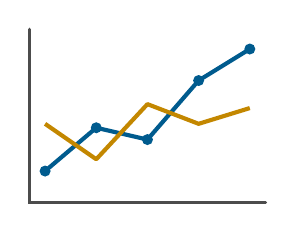
\begin{tikzpicture}[line width=0.9pt]
\draw[otgray!85!black, line width=1.2pt, line cap=round] (0,2.2) -- (0,0) -- (3,0);
  \draw[otblue!80!black, line width=1.5pt, line join=round] (0.2,0.4) -- (0.85,0.95) -- (1.5,0.8) -- (2.15,1.55) -- (2.8,1.95);
  \draw[otorange!85!black, line width=1.5pt, line join=round] (0.2,1) -- (0.85,0.55) -- (1.5,1.25) -- (2.15,1) -- (2.8,1.2);
  \foreach \x/\y in {0.2/0.4,0.85/0.95,1.5/0.8,2.15/1.55,2.8/1.95}{\fill[otblue!80!black] (\x,\y) circle[radius=0.07];}
\end{tikzpicture}
\end{document}
